% --------------------------------------
% Document Class
% --------------------------------------
\documentclass[a4paper,11pt]{article}
% --------------------------------------



% --------------------------------------
% Use Package
% --------------------------------------


\usepackage[francais]{babel}
%\usepackage{ucs}
\usepackage[utf8]{inputenc}
\usepackage[T1]{fontenc}

\usepackage{makeidx}
\usepackage{color}
\usepackage{graphicx}
\usepackage{float}
\usepackage[hidelinks]{hyperref} 
\usepackage{geometry}
%\usepackage{lastpage}
%\usepackage{marginnote}
\usepackage{fancyhdr}
%\usepackage{titlesec}
%\usepackage{framed}
\usepackage{amsmath}
\usepackage{empheq}
\usepackage{array}
\usepackage{multicol}
\usepackage{csquotes}
%\usepackage{adjustbox}

% insert code
\usepackage{listings}

% define our color
\usepackage{xcolor}

% code color
\definecolor{ligthyellow}{RGB}{250,247,220}
\definecolor{darkblue}{RGB}{5,10,85}
\definecolor{ligthblue}{RGB}{1,147,128}
\definecolor{darkgreen}{RGB}{8,120,51}
\definecolor{darkred}{RGB}{160,0,0}

% other color
\definecolor{ivi}{RGB}{141,107,185}


\lstset{
    language=java,
    captionpos=b,
    extendedchars=true,
    frame=lines,
    numbers=left,
    numberstyle=\tiny,
    numbersep=5pt,
    keepspaces=true,
    breaklines=true,
    showspaces=false,
    showstringspaces=false,
    breakatwhitespace=false,
    stepnumber=1,
    showtabs=false,
    tabsize=3,
    basicstyle=\small\ttfamily,
    backgroundcolor=\color{ligthyellow},
    keywordstyle=\color{ligthblue},
    morekeywords={include, printf, uchar},
    identifierstyle=\color{darkblue},
    commentstyle=\color{darkgreen},
    stringstyle=\color{darkred},
}


% --------------------------------------



% --------------------------------------
% Page setting
% --------------------------------------
%\pagestyle{empty}
\setlength{\headheight}{15pt}

\setcounter{secnumdepth}{3}
\setcounter{tocdepth}{2}

\makeatletter
\@addtoreset{chapter}{part}
\makeatother 

\hypersetup{         % parametrage des hyperliens
  colorlinks=true,      % colorise les liens
  breaklinks=true,      % permet les retours à la ligne pour les liens trop longs
  urlcolor= blue,       % couleur des hyperliens
  linkcolor= black,     % couleur des liens internes aux documents (index, figures, tableaux, equations,...)
  citecolor= green      % couleur des liens vers les references bibliographiques
}

% --------------------------------------

% --------------------------------------
% Information
% --------------------------------------
\title{Compte-rendu TP12 TI : Compression d'image}
\author{Elliot VANEGUE et Gaëtan DEFLANDRE}
% --------------------------------------

\definecolor{myColor}{rgb}{0.5, 0.1, 0.75}

% --------------------------------------
% Begin content
% --------------------------------------
\begin{document}

% Set language to english
  \selectlanguage{francais}

  % Start the page counting
  \pagenumbering{arabic}

  \maketitle
  
  \mbox{}
  \newpage
  \clearpage
  
  \section{Introduction}
  Le transfert et le stockage d'image sont de plus en plus fréquents et nécessitent parfois de limiter la taille
  des fichiers. Pour cela il existe des algorithmes de compression d'image, dans certains cas il faut trouver 
  un compromis entre le taux de compression et la qualité de l'image. Lors de ce TP, nous allons voir comment 
  est réalisée la compression JPEG utilisé dans le format JPG.
  
  \section{Transformée en cosinus discrète}
  La transformée en cosinus discrète est une transformation ressemblant à la transformé de Fourrier sauf
  que sa projection créé des coefficient réel. Le calcul de cette transformé nous est fournit pour une dimension.
  On peut voir que la fonction prend en paramètre un tableau à une dimension du signal que nous allons traiter.
  La sortie de la fonction est un tableau de même taille correspondant au signal transformé par la transformé 
  en cosinus discrète. Pour la fonction inverse, l'entré et la sortie de la fonction sont échangé.\\
  
  Dans un premier temps la fonction calcul les deux facteurs de normalisations $\sqrt{\frac{2}{M}}$ où M est
  la taille du signal passé en paramètre, et $c(u)$ qui vaut 1 si $u$ est différent de 0 et $\frac{1}{\sqrt{2}}$ sinon.
  Le paramètre \enquote{u} est  la position de la donné calculé. Et enfin, pour calculer une donnée la fonction
  fait la somme de toutes les autres multiplier par le cosinus de $\pi * \frac{(2m+1)*u}{2M}$ où \enquote{m}
  est la position du pixel courant.\\
  
  La propriété de séparabilité de la transformé en cosinus nous permet d'appliqué le calcul d'une dimension
  pour les deux dimensions que nous allons traiter. Ainsi, nous ne fesons que réutiliser ce calcul pour les lignes, puis pour les 
  colonnes. Nous obtenons ainsi la matrice suivante :
  
  \begin{figure}[H]
    \center
   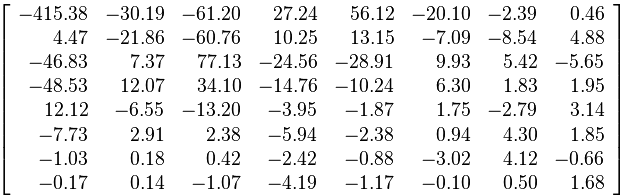
\includegraphics[width=10cm]{matrice_cosinus.png}
  \end{figure}

  Nous pouvons voir que cette matrice ne permet pas encore de réduire l'information d'une image, car aucun des 
  coefficients ne sont null. Cependant, nous remarquons que les normes des valeurs en haut à gauche de la matrice sont
  bien plus grandes que celle en bas à droite. Nous allons voir comment utiliser ce calcul pour diminuer l'information
  d'une image de beaucoup plus grande taille.
  
  \section{Utilisation de la DCT pour la compression JPEG}
  Le coût en calcul pour la transformé en cosinus discrète étant assez important, nous allons travailler sur des ROI\footnote{Region Of Interest}
  que nous allons placer dans l'image. Nous allons donc découpé l'image en 8x8, puis appliquer la transformé sur chacune de ces parties.\\
  %TODO explication roi
  
  Nous allons maintenant passer à la phase de quantification. Comme nous l'avons vu dans la partie précédente, nous avons, suite à
  l'application de la transformé en cosinus discrète, une matrice possèdant des valeurs plus importantes dans son coin supérieur
  gauche. Afin de minimiser l'imapacte de la compression sur l'image, nous allons chercher à garder les normes des valeurs les plus 
  hautes qui correspondent aux hautes fréquences. %la j'avoue que je suis pu sur. On cherche bien a garder les hautes fréquences pendant une compression?
  Nous allons donc effectuer une division bit à bit avec entre la matrice que nous avons obtenu dans la partie précédente 
  et la matrice suivante : 
  \begin{figure}[H]
    \center
   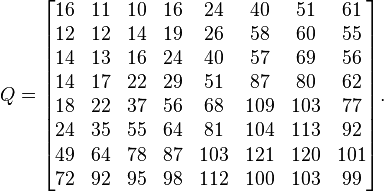
\includegraphics[width=10cm]{quantification.png}
  \end{figure}
\end{document}  